\begin{align}
\vec{x}^T\myvec{1&-1\\-1&1}\vec{x}-4\sqrt{2}a\myvec{1&1}\vec{x}=0 \label{eq:solutions/3/4/5/eq:gen}\\
\vec{V}=\myvec{1&-1\\-1&1}\implies\mydet{\vec{V}}=0,\vec{u}=\myvec{-2\sqrt{2}a\\-2\sqrt{2}a}
\end{align}
The characteristics equation of $\vec{V}$
\begin{align}
\mydet{\lambda\vec{I}-\vec{V}}=\mydet{\lambda-1&1\\1&\lambda-1}=0\\
\implies\lambda^{2}-2\lambda=0
\end{align}
The eigen values are
\begin{align}
  \lambda{_1}=0,\lambda{_2} =2
\end{align}
 The \eqref{eq:solutions/3/4/5/eq:gen} is equation of parabola as$\lambda{_1}=0 and \mydet{\vec{V}}=0.$ 
The eigen vector $\vec{p}$ is defined as
\begin{align}
    \vec{V}\vec{p}=\lambda{\vec{p}}\\
    \implies(\lambda{\vec{I}}-\vec{V})\vec{p}=0
\end{align}
for $\lambda{_1}=0$
\begin{align}
(\lambda{_1}\vec{I}-\vec{V})= \myvec{-1&1\\1&-1}\xleftrightarrow[]{R_2\rightarrow{R_2+R_1}}\myvec{-1&1\\0&0}\\\vec{p_1}=\frac{1}{\sqrt{2}}\myvec{1\\1}
\end{align}
such that $\norm{\vec{p_1}}=1$ similarly the eigen vector for $\lambda{_2}=2$ can be find
\begin{align}
    \vec{p_2}=\frac{1}{\sqrt{2}}\myvec{-1\\1}
\end{align}
\begin{align}
\vec{P}=\myvec{\vec{p_1}&\vec{p_2}}=\frac{1}{\sqrt{2}}\myvec{1&-1\\1&1}\\
\vec{D}=\myvec{\lambda_1&0\\0&\lambda_2}=\myvec{0&0\\0&2}
\end{align}
The parabola parameters are given by
\begin{align}
    f=\frac{|\eta|}{|\lambda{_2}|} ; \eta=2\vec{p_1}^T\vec{u}\\
    f= \frac{8a}{2}=4a\\
    \myvec{0 &-6\sqrt{2}a \\ 0 & 0 \\ 0 & 2}\vec{c}=\myvec{-4a\\-2\sqrt{2}a\\0\\}\\
    \vec{c}=\myvec{0\\0} where \vec{c} is vertex
\end{align}
The axes are turned around 45\degree then 
\begin{align}
    \vec{P}=\myvec{\cos\theta & -\sin\theta \\ \sin\theta & \cos\theta}\vec{x}\\
    \vec{P}=\myvec{\cos45\degree & -\sin45\degree \\ \sin45\degree & \cos45\degree}\vec{x}\\
    \vec{P} = \frac{1}{\sqrt{2}}\myvec{1&-1\\1&1}\vec{x}
\end{align}
when $\vec{P}$ passes through the \eqref{eq:solutions/3/4/5/eq:gen} we get
\begin{multline}
\begin{aligned}
\vec{x}^T\frac{1}{\sqrt{2}}\myvec{1&1\\-1&1}\myvec{1&-1\\-1&1}\frac{1}{\sqrt{2}}\myvec{1&-1\\1&1}\vec{x}\\-4\sqrt{2}a\myvec{1&1}\frac{1}{\sqrt{2}}\myvec{1&-1\\1&1}\vec{x}=0
\end{aligned}
\end{multline}
\begin{align}
    \vec{x}^T\myvec{0&0\\0&2}\vec{x}-4a\myvec{2&0}\vec{x}=0\\
    \vec{V}=\myvec{0&0\\0&2}\implies\mydet{\vec{V}}=0
\end{align}
Therefore it is parabola..
\begin{figure}[!ht]
\centering
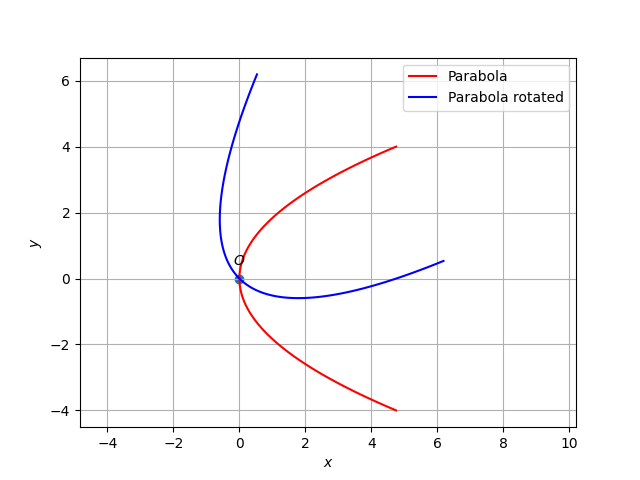
\includegraphics[width=\columnwidth]{./solutions/3/4/5/parabola.png}
\caption{ parabola with $a$ =1}
\label{eq:solutions/3/4/5/Fig}
\end{figure}
